\documentclass[border=20pt, tikz]{standalone}
\usetikzlibrary{shapes.geometric, arrows.meta, positioning, calc, backgrounds}

\begin{document}
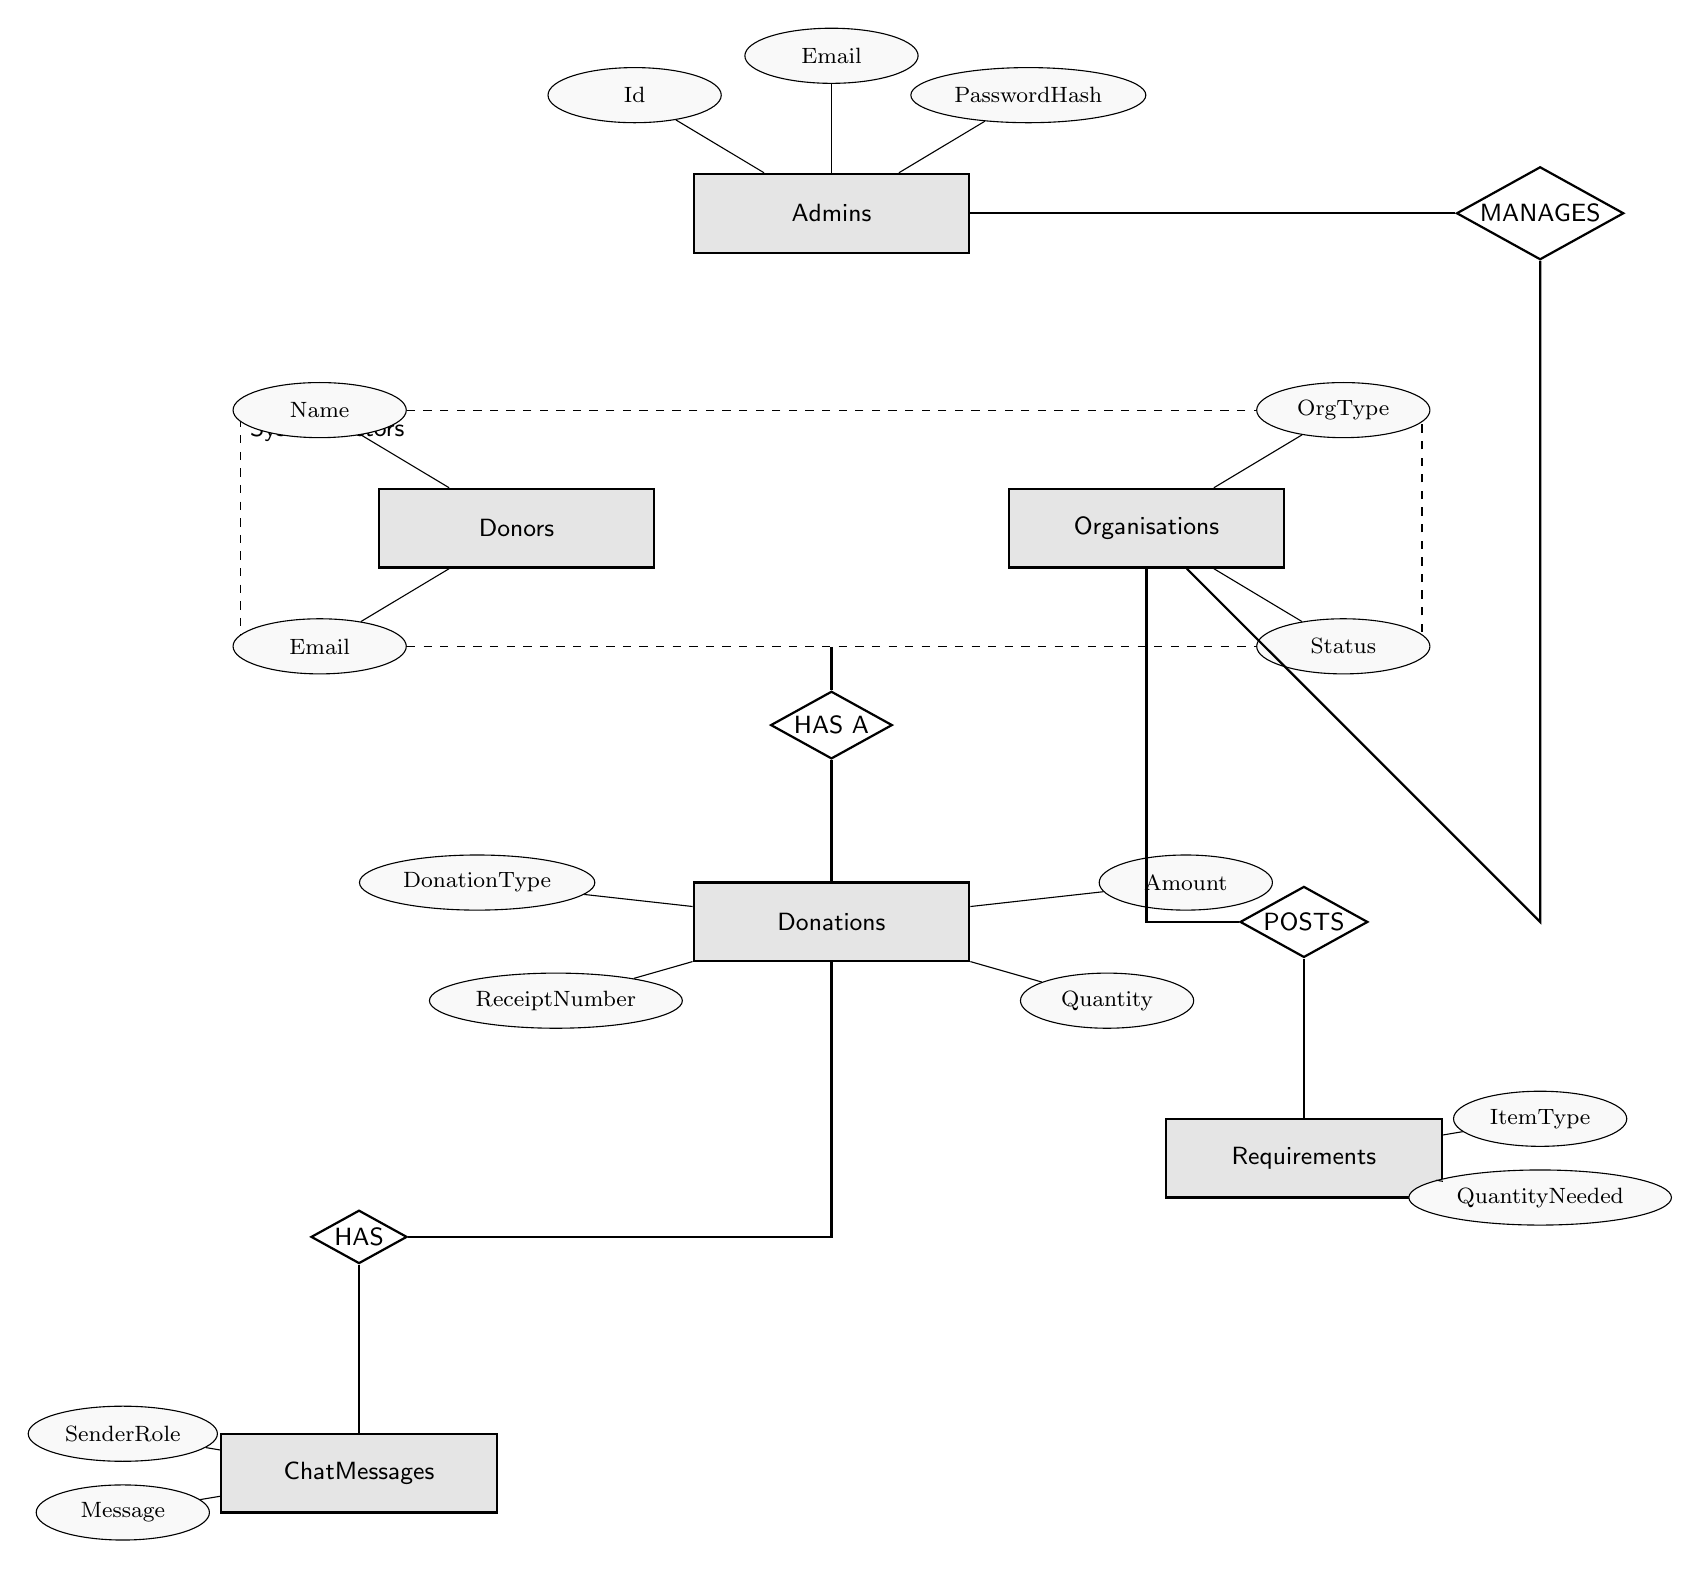
\begin{tikzpicture}[
    font=\sffamily\small,
    entity/.style={
        rectangle, draw=black, thick, 
        fill=gray!20, 
        minimum width=3.5cm, minimum height=1cm, align=center
    },
    attribute/.style={
        ellipse, draw=black, thin, 
        fill=gray!5, 
        minimum width=2.2cm, minimum height=0.7cm, align=center, font=\footnotesize
    },
    relationship/.style={
        diamond, draw=black, thick, 
        fill=white, 
        aspect=1.8, align=center, inner sep=1pt
    },
    isa/.style={
        draw, regular polygon, regular polygon sides=3, 
        minimum size=1.2cm, fill=white, thick, align=center, inner sep=0pt
    },
    line/.style={draw=black, thick}
]

% 1. TOP SECTION: Admin & Actors
\node[entity] (Admin) at (0, 7) {Admins};
\node[attribute] (A1) at (-2.5, 8.5) {Id};
\node[attribute] (A2) at (0, 9) {Email};
\node[attribute] (A3) at (2.5, 8.5) {PasswordHash};
\draw (Admin) -- (A1); \draw (Admin) -- (A2); \draw (Admin) -- (A3);

% Actors Box
\begin{scope}[on background layer]
    \node[draw, dashed, rectangle, inner sep=0.8cm] (ActorBox) at (0, 3) [minimum width=15cm, minimum height=3cm] {};
    \node[anchor=north west] at (ActorBox.north west) {System\_Actors};
\end{scope}

\node[entity] (Donor) at (-4, 3) {Donors};
\node[entity] (Org) at (4, 3) {Organisations};

% Actor Attributes
\node[attribute] (D1) at (-6.5, 4.5) {Name};
\node[attribute] (D2) at (-6.5, 1.5) {Email};
\draw (Donor) -- (D1); \draw (Donor) -- (D2);

\node[attribute] (O1) at (6.5, 4.5) {OrgType};
\node[attribute] (O2) at (6.5, 1.5) {Status};
\draw (Org) -- (O1); \draw (Org) -- (O2);

% 2. CENTER SECTION: Donations
\node[relationship] (Rel1) at (0, 0.5) {HAS A};
\draw[line] (ActorBox.south) -- (Rel1);

\node[entity] (Donation) at (0, -2) {Donations};
\draw[line] (Rel1) -- (Donation);

% Donation Attributes
\node[attribute] (Do1) at (-3.5, -3) {ReceiptNumber};
\node[attribute] (Do2) at (-4.5, -1.5) {DonationType};
\node[attribute] (Do3) at (3.5, -3) {Quantity};
\node[attribute] (Do4) at (4.5, -1.5) {Amount};
\draw (Donation) -- (Do1); \draw (Donation) -- (Do2); \draw (Donation) -- (Do3); \draw (Donation) -- (Do4);

% 3. BOTTOM SECTION: Requirements & Chat
\node[relationship] (RelReq) at (6, -2) {POSTS};
\draw[line] (Org) |- (RelReq);

\node[entity] (Requirement) at (6, -5) {Requirements};
\draw[line] (RelReq) -- (Requirement);

\node[attribute] (R1) at (9, -4.5) {ItemType};
\node[attribute] (R2) at (9, -5.5) {QuantityNeeded};
\draw (Requirement) -- (R1); \draw (Requirement) -- (R2);

\node[relationship] (RelMsg) at (-6, -6) {HAS};
\draw[line] (Donation) |- (RelMsg);

\node[entity] (Message) at (-6, -9) {ChatMessages};
\draw[line] (RelMsg) -- (Message);

\node[attribute] (M1) at (-9, -8.5) {SenderRole};
\node[attribute] (M2) at (-9, -9.5) {Message};
\draw (Message) -- (M1); \draw (Message) -- (M2);

% Admin Manages link
\node[relationship] (RelAdm) at (9, 7) {MANAGES};
\draw[line] (Admin) -- (RelAdm);
\draw[line] (RelAdm) -- (9, -2) -- (Org); % Admin manages organisations/approval

\end{tikzpicture}
\end{document}
